\section{Directory Structure}
\begin{center}
  \begin{figure}[H]
  \centering
  %\vspace*{5\baselineskip}
  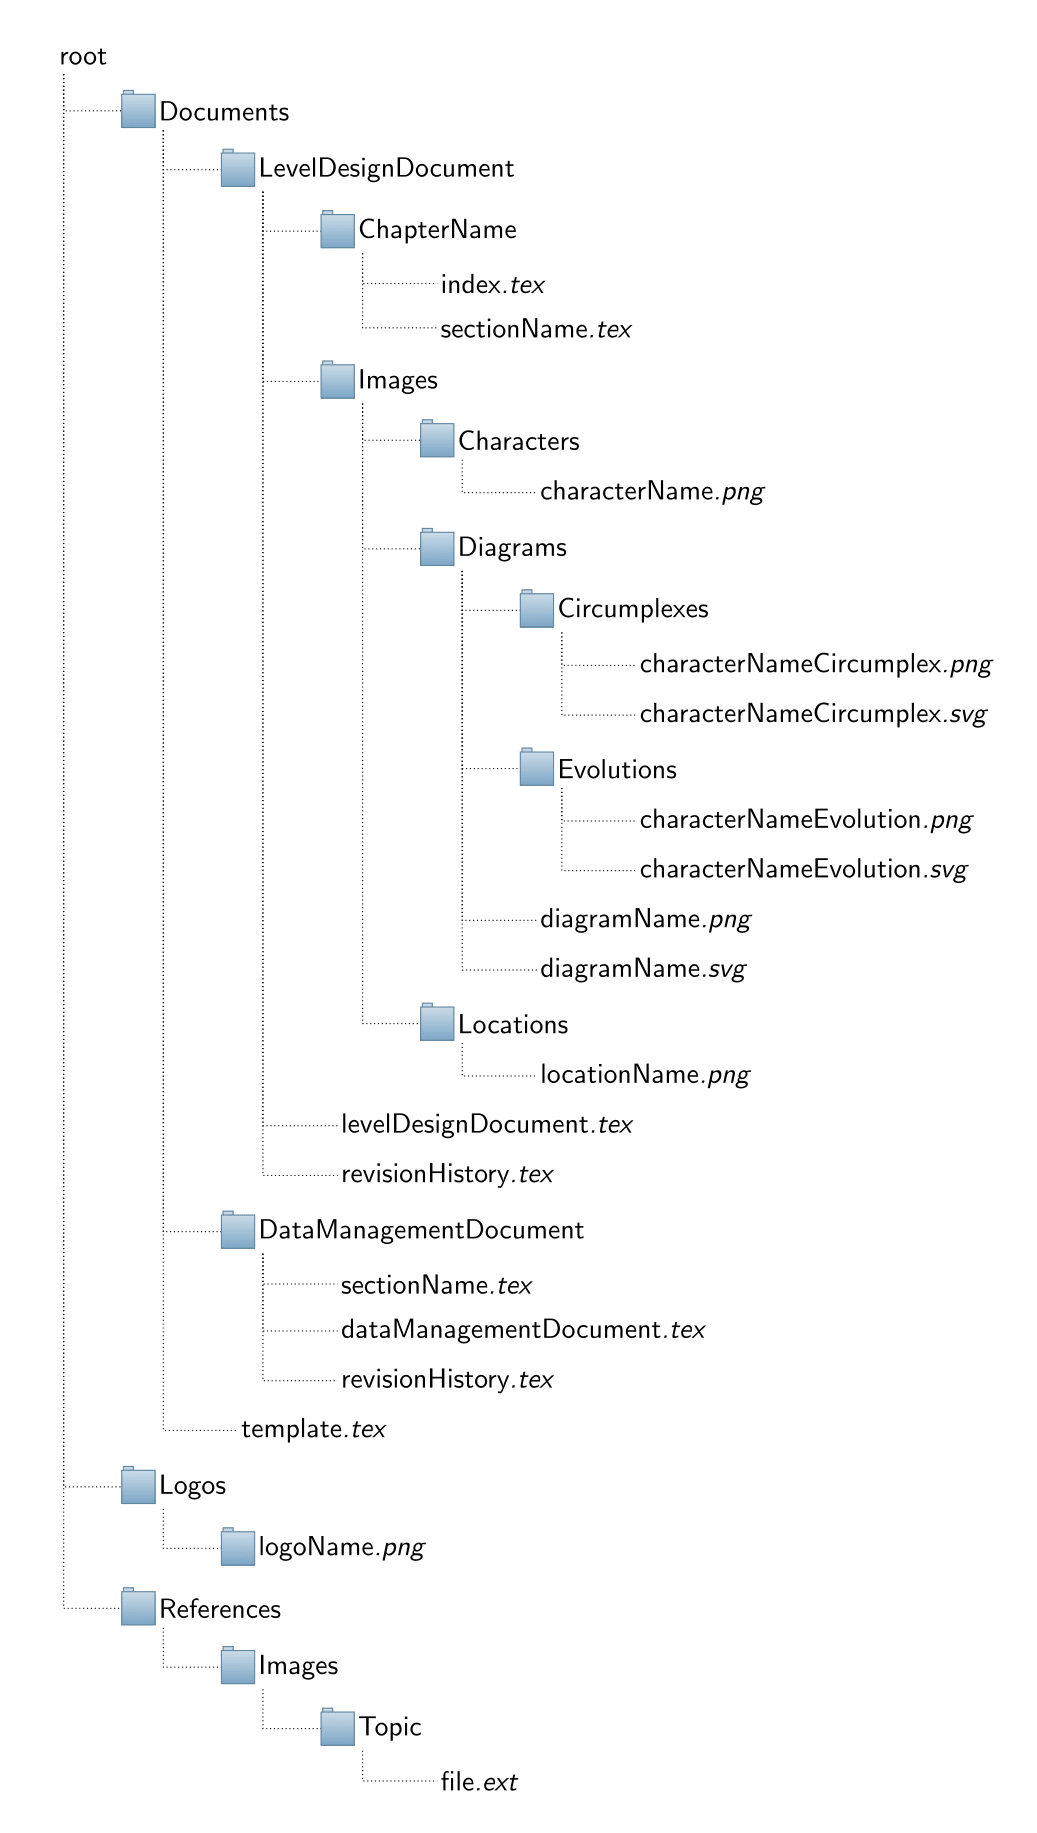
\includegraphics[width=10cm]{directories}
  \end{figure}
\end{center}
\begin{itemize}
\item \textbf{\path{./Documents}}: contains a directory for each document and a template that has to be used for eventual new documents.
  \begin{itemize}
    \item \textbf{\path{./DataManagmentDocument}}: contains the data managment document, where you find all technical features and rules to work on the project, and the relative revision history.

    \item \textbf{\path{./LevelDesignDocument}}: contains the level design document, where you find everything about the game and level, the relative revision history, a directory containing images for the whole project and a directory for each chapter. Each chapter subfolder has its own section files and a "index.tex" file.
    \begin{itemize}
    \item \textbf{\path{./Images}}: contains every image for the level design documentation. There are some subfolders:
    \begin{itemize}
      \item \textbf{\path{/Characters}}: contains one portrait for each character.
      \item \textbf{\path{/Diagrams}}: contains all diagrams file used in the level design document. If the diagram is a circumplex or an evolution it has to be placed in the relative subfolder.
        \item \textbf{\path{/Locations}}: contains one picture for each location.
        \item \textbf{\path{/Maps}}: contains all the maps used in the level design document.
    \end{itemize}
\end{itemize}
\end{itemize}
    \item \textbf{\path{./Logos}}: contains all the logos (\textit{.png} file) used in the level design document.

    \item \textbf{\path{./ReferenceImages}}: this directory contains all the LaTeX files about the story.

\end{itemize}

